\pagebreak
\subsection{Task 2 - Building and Configuring the Server Array}

\subsubsection*{Download Windows Server 2016 ISO}
\begin{enumerate}[series=task2methodology1]
  \item Download Windows Server 2016 from the `Microsoft Imagine' website, as shown in Figure~\ref{fig:task2:winserver2016_download} in the \nameref{app:ancillaryscreenshots} appendix.
\end{enumerate}

\noindent I have taken a different approach for the next step to the normal approach of uploading the ISO via the vSphere Web Client or vSphere Client (desktop). This is due to a bug with ESXi 6.0.0 that prevents uploads when using the IPv6 address to access the instance's Web Client interface. When you use the `Datastore Browser' to upload a file, the upload freezes at 0\% and does not progress at all.

\subsubsection*{Transfer the ISO into the ESXi instance}
\begin{enumerate}[resume*=task2methodology1]
  \item Use the Web Client to enable SSH access to the ESXi instance by going to `Host > Actions > Services > Enable Secure Shell (SSH)'.
  \item Download \texttt{pscp.exe} from the PuTTY website\footnote{\url{https://www.chiark.greenend.org.uk/~sgtatham/putty/latest.html}}.
  \item In the Web Client, find the path to `datastore1' by going to `Storage > datastore1' and viewing the `Location`. In my case, this was:\\ \texttt{/vmfs/volumes/5af1d3e9-abd56f67-0cdf-000c296b7530/}.
  \item On the workstation host where the ISO was downloaded, in PowerShell from the directory that the ISO resides in run:\\
  \texttt{C:\textbackslash tools\textbackslash pscp.exe -6}\\
  \texttt{.\textbackslash 14393.0.161119-1705.RS1\_REFRESH\_SERVER\_EVAL\_X64FRE\_EN-US.ISO}\\
  \texttt{root@[fe80::20c:29ff:fe6b:7530]:}\\
  \texttt{/vmfs/volumes/5af1d3e9-abd56f67-0cdf-000c296b7530/isos}\\
  This will secure copy the ISO to the ESXi instance over SSH.
\end{enumerate}

\noindent When not using the SSH service for remote administration, it should be disabled to reduce the attack surface of the ESXi instance. It should be noted that restarting the ESXi instance will automatically re-disable the SSH service.

\subsubsection*{Set up an Active Directory Domain Controller}
\begin{enumerate}[series=task2methodology2]
  \item Create a new VM in the Web Client for the ESXi instance. Notable steps are detailed forthwith:
    \begin{enumerate}[label=(\alph*)]
      \item Select `Create a new virtual machine` in the `Select creation type` step.
        \begin{figure}[H]
          \centering
          \captionsetup{skip=2pt}
          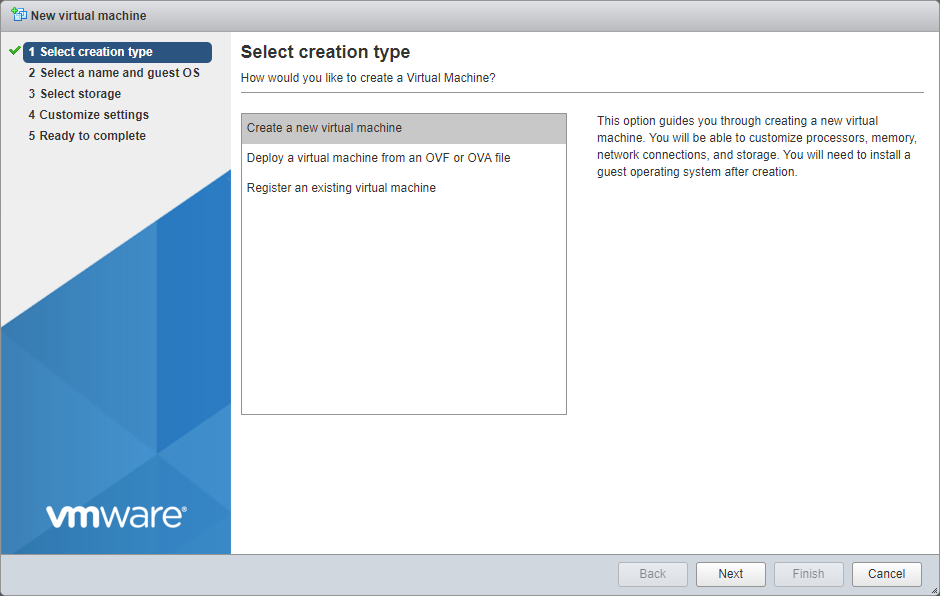
\includegraphics[width=\textwidth]{task2_06_winserver2016_2_dc_crop}
          \caption{Creating a new VM in ESXi}
          \label{fig:task2:vspherewc_newvm1}
        \end{figure}
      \item Give the VM a unique (within the ESXi instance) name and set the Guest OS Family and Version to be `Windows` and `Microsoft Windows Server 2016 (64-bit)` respectively.
        \begin{figure}[H]
          \centering
          \captionsetup{skip=2pt}
          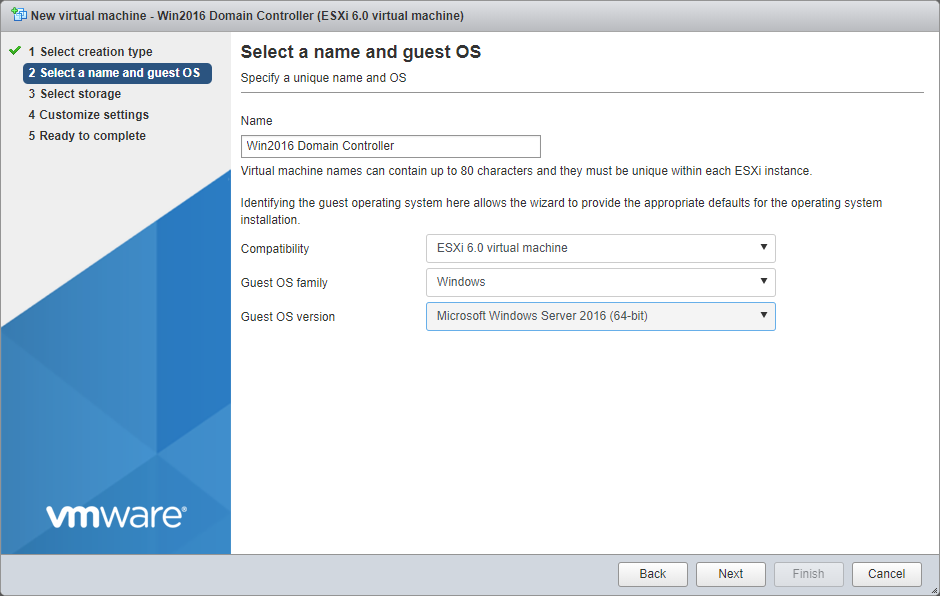
\includegraphics[width=\textwidth]{task2_06_winserver2016_3_dc_crop}
          \caption{Selecting the name and guest OS in the `New virtual machine` wizard}
          \label{fig:task2:vspherewc_newvm2}
        \end{figure}
      \item Mount the Windows Server 2016 ISO in the CD drive for the new virtual machine.
      \begin{figure}[H]
        \centering
        \captionsetup{skip=2pt}
        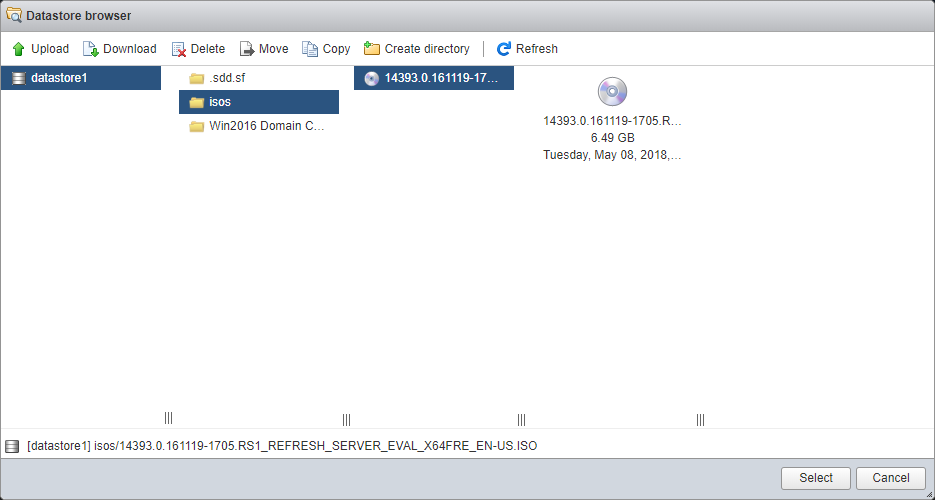
\includegraphics[width=\textwidth]{task2_06_winserver2016_9_dc_crop}
        \caption{Selecting the ISO to run at boot in the new VM}
        \label{fig:task2:vspherewc_newvm3}
      \end{figure}
    \end{enumerate}
\end{enumerate}

\noindent The screenshot in Figure~\ref{fig:task2:vspherewc_newvm4} in the \nameref{app:ancillaryscreenshots} appendix shows the Web Client UI display for the newly created VM.\\\\
\noindent For the next steps, I used the vSphere Client to display the console of specific VMs inside ESXi. This is primarily because of a bug in ESXi 6.0 that prevents consoles from being shown in the browser, as shown in Figures~\ref{fig:task2:vspherewc_bug1} and~\ref{fig:task2:vspherewc_bug2} in the \nameref{app:ancillaryscreenshots} appendix. However, the vSphere Client is also nicer to use as it responds faster and does not attempt to scale the console to the size of the browser window.

\begin{enumerate}[resume*=task2methodology2]
  \item x
\end{enumerate}

\subsubsection*{Set up a User Server}
\subsubsection*{Create a failover configuration}
